\begin{align}
\begin{split}
\vec{P}=\frac{\vec{A+B}}{2}=\myvec{-1 & \frac{3}{2}} \\ 
\vec{Q}=\frac{\vec{B+C}}{2}=\myvec{2 &4 }  \\ 
\vec{R}=\frac{\vec{C+D}}{2}=\myvec{5 & \frac{3}{2}}  \\ 
\vec{S}=\frac{\vec{A+D}}{2}=\myvec{2 & -1}  
\end{split}
\label{eq:solutions/quad/1/eqn} 
\end{align}

$\because$
\begin{align}
\frac{\vec{P+R}}{2} = \frac{\vec{Q+S}}{2}=\frac{1}{2}\myvec{4 \\ 3} 
%\label{eq:solutions/quad/1/eqn}
\end{align} 
PQRS is a parallelogram.
\begin{align}
(\vec{P-R})=\myvec{-6 & 0} 
(\vec{Q-S})=\myvec{0\\5} 
%\label{eq:solutions/quad/1/eqn}
\\
\end{align}

\begin{align}
(\vec{P-R})^T(\vec{Q-S}) = \begin{pmatrix}-6 & 0\end{pmatrix}
\begin{pmatrix} 0 \\ 5 \end{pmatrix} 
%\label{eq:solutions/quad/1/eqn}
\\
(\vec{P-R})^T(\vec{Q-S})=\myvec{0}
\\  
%\label{eq:solutions/quad/1/eqn}
\end{align}
Diagonal bisect orthogonally. 
Thus, PQRS is a rhombus.  Se Fig. \ref{eq:solutions/quad/1/fig:Simulation of midpoint of ABCD form PQRS}

\begin{figure}[htbp]
\centering 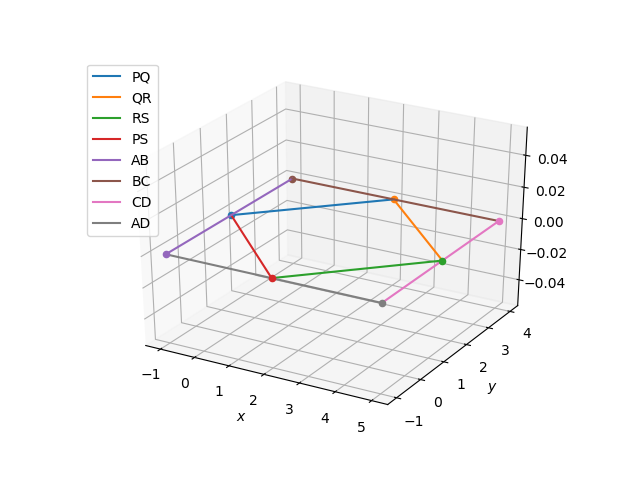
\includegraphics[width=\columnwidth]{./solutions/quad/1/Figure_1.png}
\caption{Simulation of midpoint of ABCD forms PQRS.}
\label{eq:solutions/quad/1/fig:Simulation of midpoint of ABCD form PQRS}
\end{figure}



\textbf{Step4}: We will check whether Parallelogram PQRS is Square or not.
\begin{align}
(\vec{P-Q})=\frac{1}{2}\myvec{-6 \\-5} 
%\label{eq:solutions/quad/1/eqn}
\\
(\vec{P-S})=\frac{1}{2}\myvec{-6\\5} 
%\label{eq:solutions/quad/1/eqn}
\\
\end{align}
If adjacent side of parallelogram are orthogonal to each other then PQRS is a Square.
\begin{align}
(\vec{P-Q})^T(\vec{P-S})=\frac{1}{4}\myvec{-6 & -5}\myvec{-6 \\ 5} \ne = 0 
%\label{eq:solutions/quad/1/eqn}
%\\
\end{align}
Here the angle between adjacent side is not 90 $^{\circ}$.
Hence, PQRS is not a Square.
